\documentclass{nordic}
\usepackage[utf8]{inputenc} % In case one needs to specify character encoding
\usepackage{graphicx}
\usepackage{amsmath}
\usepackage[colorlinks=true,linkcolor=black,citecolor=black,urlcolor=black]{hyperref}

\usepackage{tensortyping}
\usepackage{pgfplots}
\usepgfplotslibrary{patchplots}
\usepgfplotslibrary{groupplots}
%\usepgfplotslibrary{external}
\pgfplotsset{compat=1.3}% do not forget this!

\newcommand{\NSCM}{23}
\newcommand{\submissionyear}{2010}
\newcommand{\submissiondate}{September 20th 2010}
\newcommand{\submissionpage}{http://congress.cimne.upc.es/nscm-\NSCM/frontal}

\header{
  \NSCM rd Nordic Seminar on Computational Mechanics\\
  NSCM-\NSCM\\
  A. Eriksson and G. Tibert (Eds)\\
  \copyright KTH, Stockholm, \submissionyear
}

\title{Multiscale Modeling of Sintering of Hard Metal}

\author{Mikael Öhman$^*$, Kenneth Runesson and Fredrik Larsson}

\heading{Mikael Öhman, Kenneth Runesson and Fredrik Larsson}

\address{%
Department of Applied Mechanics\\
Chalmers University of Technology\\
Gothenburg, Sweden\\
e-mail: \url{mikael.ohman@chalmers.se}, web page: \url{http://www.chalmers.se/am/EN/}
}

\keywords{Sintering, Sintering stress, Surface tension, Homogenization, FE$^2$}

\abstract{%
In this contribution, we discuss the multiscale modeling of sintering of hard metal, which is composed of hard particles (WC) with a melted binder (Co).
Numerical results are shown for a coupled FE$^2$ analysis involving homogenization of the consolidating compact.
%which shows complex sintering phenomena with only two material parameters.
}

\begin{document}
\maketitle

\section{INTRODUCTION}
The sintering phenomenon on the mesoscale is driven by surface tension on the melted binder, and
the homogenized effect of the surface tension is the so-called sintering stress.
From the macroscopic perspective, the specimen (green body) shrinks due to this volumetric sintering stress. In the case of inhomogeneous
initial density in the green body, the sintering can result in unwanted final deformations.
%On the mesoscale, particles are merged, driven by the surface tension on the free pore surface.

\section{THEORY}
Finite elements and computational homogenization have been applied to a Representative Volume Element (RVE) of the mesoscale.
The melted binder is modeled as a Stokes flow, with surface tension potential energy on the free surface. Hard inclusions are modeled by applying a high viscosity.
%This is coupled to the macroscopic stress and strain and the mesoscale  is solved for every time step in every integration point.
Different choices of boundary conditions are available on the RVE for the prolongation.
The advantage of the multiscale approach is that it can capture the complex behavior of sintering with simple material models with measurable parameters.

The surface tension load can be expressed by a traction $\to t$ on the free surface as
\begin{gather}
 \to t = 2\kappa\gamma \to n
\end{gather}
where $\kappa$ is the Gaussian curvature of the surface, $\gamma$ is the surface tension coefficient and $\to n$ is the surface normal. %\cite{sintering}.
Since the traction is geometry dependent, a tangent with respect to the displacement also appears in the equations.
Using the divergence theorem one can avoid the second derivative in the FE-formulation,
but the incompressible Stokes flow requires higher order basis functions.

For the homogenization, extra care has to be placed on the formulation to fulfill the Hill-Mandel condition.
Since the internal boundary potential on the mesoscale gives rise to a discontinuous stress,
the common derivations for stress/strain homogenization do not apply directly.

%SHOULD I INCLUDE SOME MATH? IT IS WAY TO MUCH TO GO THROUGH EVERYTHING?!

\section{PRELIMINARY RESULTS}
Numerical examples are evaluated for a 2D, fully coupled, FE$^2$ problem as a proof of concept.
Taylor-Hood elements for the linear Stokes flow, and quadratic edge elements for the surface tension, are employed for the mesoscale analysis.
Linear triangular elements with one integration point are used on the macroscopic scale.
Dirichlet boundary conditions are used for the prolongation of the macroscopic strain rate.
The geometry is deformed at the end of each time step in the framework of an updated Lagrangian formulation.
The model contains only two material parameters, the viscosity $\nu$ and the surface tension $\gamma$,
both set to unit value as they will only scale the linear response.

The finite elements for both meso- and macroscale have been implemented in the open source finite element code OOFEM\cite{OOFEM},
and extensions will be available in future releases. The multiscale step is carried out by implementing a special constitutive driver for the macroscopic scale.
This driver calls and solves a subscale finite element problem for the given macroscale strain, whereafter the homogenized stress is calculated.
This approach fits cleanly into the OOFEM framework, and could be used to recursively perform any number of multiscale computations.

\begin{figure}[hbpt]
 \centering
 \begin{tikzpicture}
  \begin{groupplot}[
    group style={group size=3 by 1},
    width=5cm,
    height=5cm,
    xticklabels={},
    yticklabels={},
    %colormap/cool,
    patch to triangles,
    %patch refines=1,
	%shader=interp,
	%shader=flat,
    %colorbar style={y=Pressure,title=Colorbar},
   point meta min={-1.6}, % Had to look them manually. Might be possible to fetch from the first plot though.
   point meta max={1.16}
   ]
  \nextgroupplot
  \addplot[patch,patch table={figures/connectivity_tri2.dat},patch type=triangle quadr, ultra thin, point meta=\thisrow{p}]
    table[x=x,y=y] {figures/nodes_1.dat};
  \addplot[patch,mesh,patch table={figures/connectivity_edge.dat},patch type=quadratic spline, thick, draw=black]
    table[x=x,y=y] {figures/nodes_1.dat};
  \nextgroupplot%[xtick=\emtpy]
  \addplot[patch,patch table={figures/connectivity_tri2.dat},patch type=triangle quadr, ultra thin, point meta=\thisrow{p}]
    table[x=x,y=y] {figures/nodes_50.dat};
  \addplot[patch,mesh,patch table={figures/connectivity_edge.dat},patch type=quadratic spline, thick, draw=black]
    table[x=x,y=y] {figures/nodes_50.dat};
  \nextgroupplot[colorbar,colorbar right, colorbar style={ylabel=Pressure}]
  \addplot[patch,patch table={figures/connectivity_tri2.dat},patch type=triangle quadr, ultra thin, point meta=\thisrow{p}]
    table[x=x,y=y] {figures/nodes_200.dat};
  \addplot[patch,mesh,patch table={figures/connectivity_edge.dat},patch type=quadratic spline, thick, draw=black]
    table[x=x,y=y] {figures/nodes_200.dat};
  \end{groupplot}
  \draw[thick,black,->,shorten >=5pt,shorten <=5pt] (group c1r1.east) -- (group c2r1.west);
  \draw[thick,black,->,shorten >=5pt,shorten <=5pt] (group c2r1.east) -- (group c3r1.west);
 \end{tikzpicture}
 \caption{Evolution of the free surface within an RVE and the corresponding pressure field}\label{fig:rve_evolution}
\end{figure}
The first example, shown in Figure \ref{fig:rve_evolution}, concerns an RVE at a single macroscale integration point.
The outer boundary is fully prescribed and the liquid/binder-pore surface can be seen to evolve.
The negative pressure is represented as the sintering stress on the macroscale.

\begin{figure}[htpb]
 \centering
 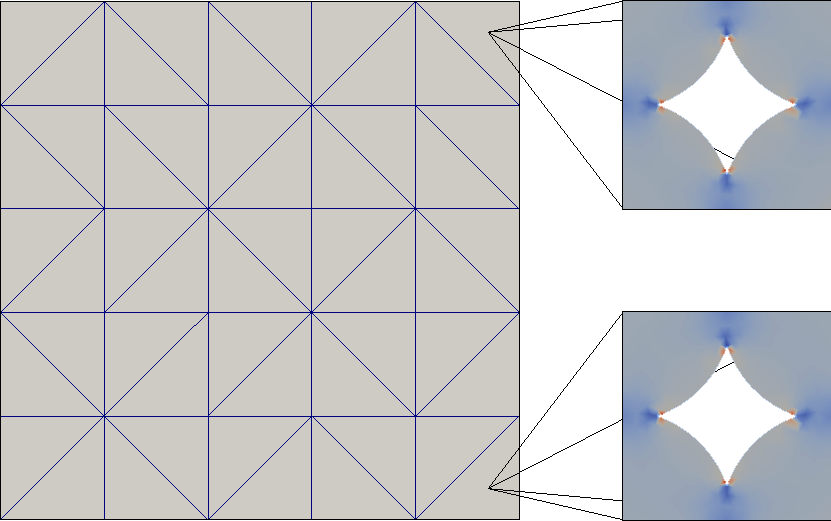
\includegraphics[width=0.43\textwidth]{figures/Sintering_5x5_000.png}
 \begin{tikzpicture}
  \draw[thick,black,->] (0,0) -- (0.5,0); \draw[use as bounding box] (0,-2.1);
 \end{tikzpicture}
 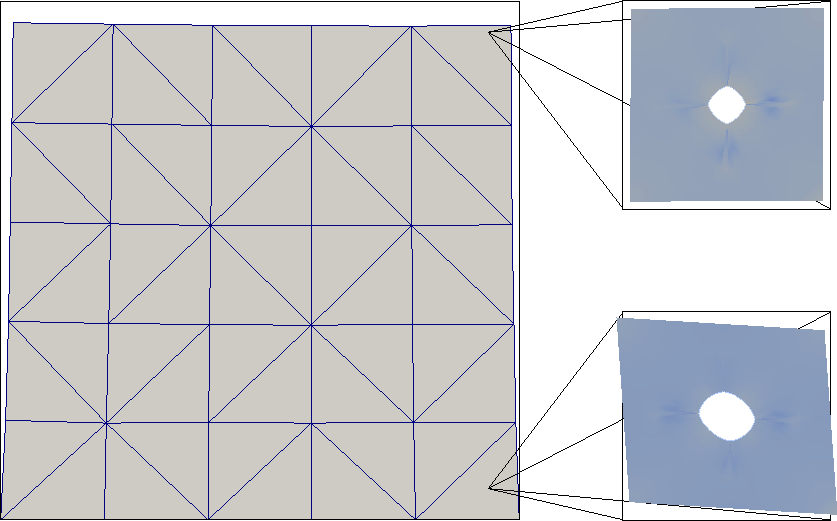
\includegraphics[width=0.43\textwidth]{figures/Sintering_5x5_114.png}
 \caption{FE$^2$ analysis of the constrained sintering of a specimen; ``snapshots`` of two RVE's at the start and end of the process.}\label{fig:multiscale}
\end{figure}

The second example concerns a coupled FE$^2$-analysis, shown in Figure \ref{fig:multiscale}, where the lower boundary has been fully prescribed.
%Since the volume fraction at its lowest still reaches around 0.84 in a 2D-model, this  means a very limited change in volume on the macro scale.
Since the initial density can never go lower than around 0.84 in a 2D representation of this microstructure, the possible macroscale volume change is quite limited.

\section{DISCUSSION}
%The natural extension of this work is to bring this model into 3D.
A major obstacle is the representation of the evolving geometry.
Remeshing is required to keep a nice representation despite topological changes.
To keep track of the multiple boundaries, level sets are commonly used in free surface flows.
% Such an extension is planned to be included in a future version of OOFEM.

\bibliography{references_extended}
\bibliographystyle{naturemag}
%\bibliographystyle{plain}

\end{document}

